\section{Iteracyjne metody rozwiązywania równań eliptycznych}

Będziemy korzystać z równania:

$$u_{i,j} = \frac{1}{4}(u_{i+1,j} + u_{i-1,j} + u_{i,j+1} + u_{i,j-1}) - \frac{1}{4}h^2f_{i,j}$$

\vspace{0.5cm}

Rozpatrzmy równanie:

\[
\begin{cases}
\vspace{0.1cm} 
\hspace{0,1cm}\frac{\delta^2 u}{\delta x^2} + \frac{\delta^2 u}{\delta y^2} = f\\
\vspace{0.1cm}
\hspace{0,1cm}u_{|\delta \Omega} = \overline{u} \\
\end{cases}
\]

, gdzie:

$(x,y) \in \Omega$

$\Omega = [a,b] \times [c,d]$

$\Omega \subset \Re^2$

\subsection{Cel ćwiczenia}

Naszym zadaniem było stworzenie algorytmu rozwiązującego następujące równania:

a) \hspace{6cm} b)

$\frac{\delta^2 u}{\delta x^2} + \frac{\delta^2 u}{\delta y^2} = 0$ \hspace{4.15cm} $\frac{\delta^2 u}{\delta x^2} + \frac{\delta^2 u}{\delta y^2} = -cos(x+y)-cos(x-y)$

, gdzie: \hspace{5.2cm} , gdzie:

warunki brzegowe: \hspace{3.5cm} warunki brzegowe:

$u(x,0) = 2lnx$ \hspace{4.15cm} $u(x,0) = cos(x)$

$u(1,y) = ln(y^2 + 1)$ \hspace{3.3cm} $u(0,y) = cos(y)$

$u(x,1) = ln(x^2 + 1)$ \hspace{3.28cm} $u(x,\frac{\pi}{2}) = 0$

$u(2,y) = ln(y^2 + 4)$ \hspace{3.3cm} $u(\pi,y) = -cos(y)$

rozwiązanie analityczne: \hspace{2.6cm} rozwiązanie analityczne:

$u(x,y) = ln(x^2 + y^2)$ \hspace{3.1cm} $u(x,y) = cos(x)\cdot cos(y)$

\vspace{0.5cm}

Trzema metodami: Jacobiego, Gaussa $-$ Seidela oraz nadrelaksacji Younge'a. Dodatkowo przedstawimy dwupoziomową metodę Peacemanna $-$ Rachforda.

\subsection{Metoda Jacobiego}

W metodzie tej wybieramy pierwsze arbitralne, dowolne przybliżenie rozwiązania numerycznego.

Im bliżej rozwiązania analitycznego dobrane jest przybliżenie tym mniej iteracji będziemy potrzebować w procesie iteracyjnym.

Jedna pełna iteracja polega na poprawieniu jeden raz wartości przybliżonych we wszystkich węzłach wewnętrznych siatki, aby następnie przejść do kolejnej iteracji wychodząc z tego samego węzła co poprzednio.

Dobór punktów nie ma znaczenia, ważne jest jedynie aby w kolejnych iteracjach zachować obrany porządek.

Zaletą metody Jacobiego jest nie generowanie wielkich macierzy; wadą dość wolna zbieżność.

Dowolne pierwsze przybliżenie:

$$u_{i,j}^{(n)} = \frac{1}{4}(u_{i+1,j}^{(n)} + u_{i-1,j}^{(n)} + u_{i,j+1}^{(n)} + u_{i,j-1}^{(n)}) - \frac{1}{4}h^2f_{i,j}$$

\subsection{Algorytm}

a)

//kod z jacobi1

b)

//kod z jacobi1

\subsection{Wykresy}

a)

Dla n = 5:

\begin{figure}[!ht]
	\begin{center}
		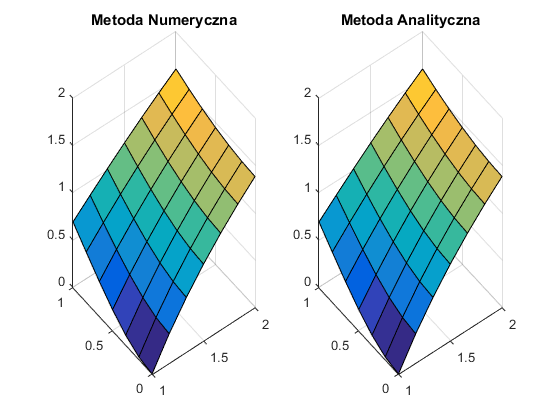
\includegraphics[width=0.8\textwidth]{Lab6/charts/jacobi/zad1/5.png}
	\end{center}
\end{figure}

Liczba wykonanych iteracji $ = 38 $

Czas wykonywania algorytmu $ = 0.177 s$

\newpage

Dla n = 15:

\begin{figure}[!ht]
	\begin{center}
		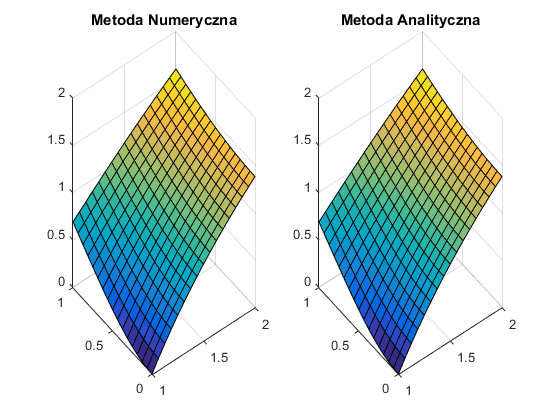
\includegraphics[width=0.8\textwidth]{Lab6/charts/jacobi/zad1/15.png}
	\end{center}
\end{figure}


Liczba wykonanych iteracji $ = 170 $

Czas wykonywania algorytmu $ = 0.202 s$

Dla n = 30:

\begin{figure}[!ht]
	\begin{center}
		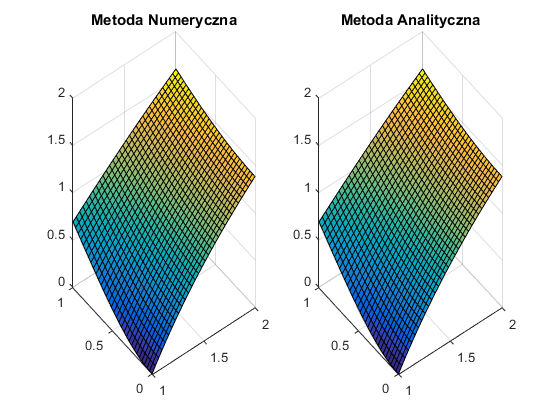
\includegraphics[width=0.8\textwidth]{Lab6/charts/jacobi/zad1/30.png}
	\end{center}
\end{figure}

Liczba wykonanych iteracji $ = 415 $

Czas wykonywania algorytmu $ = 0.289 s$

\newpage

Dla n = 50:

\begin{figure}[!ht]
	\begin{center}
		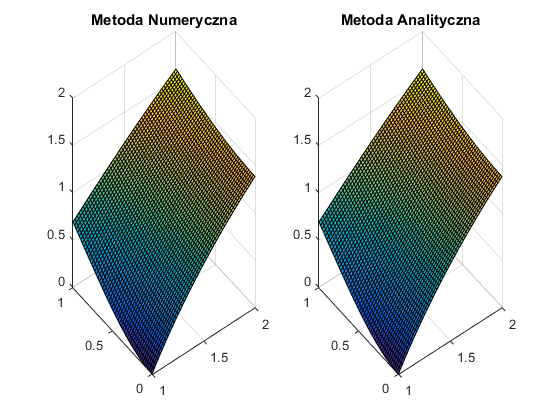
\includegraphics[width=0.8\textwidth]{Lab6/charts/jacobi/zad1/50.png}
	\end{center}
\end{figure}

Liczba wykonanych iteracji $ = 797 $

Czas wykonywania algorytmu $ = 0.777 s$

b)

Dla n = 5:

\begin{figure}[!ht]
	\begin{center}
		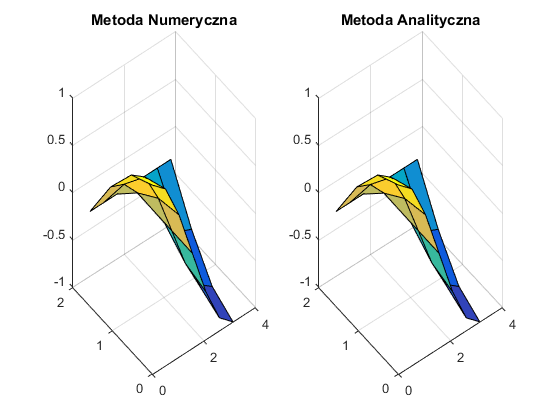
\includegraphics[width=0.8\textwidth]{Lab6/charts/jacobi/zad2/5.png}
	\end{center}
\end{figure}

Liczba wykonanych iteracji $ = 23 $

Czas wykonywania algorytmu $ = 0.175 s$

Dla n = 15:

\begin{figure}[!ht]
	\begin{center}
		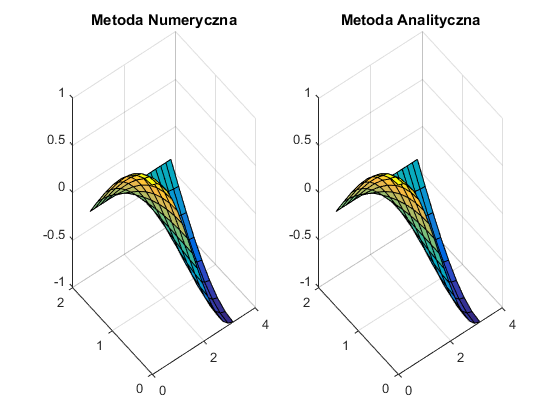
\includegraphics[width=0.8\textwidth]{Lab6/charts/jacobi/zad2/15.png}
	\end{center}
\end{figure}

Liczba wykonanych iteracji $ = 138 $

Czas wykonywania algorytmu $ = 0.179 s$

Dla n = 35:

\begin{figure}[!ht]
	\begin{center}
		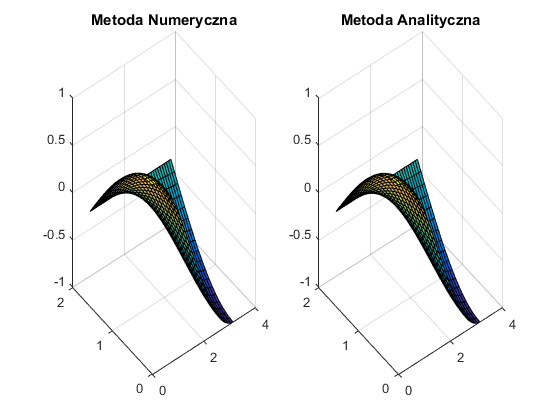
\includegraphics[width=0.8\textwidth]{Lab6/charts/jacobi/zad2/35.png}
	\end{center}
\end{figure}

Liczba wykonanych iteracji $ = 529 $

Czas wykonywania algorytmu $ = 0.294 s$

\newpage

Dla n = 55:

\begin{figure}[!ht]
	\begin{center}
		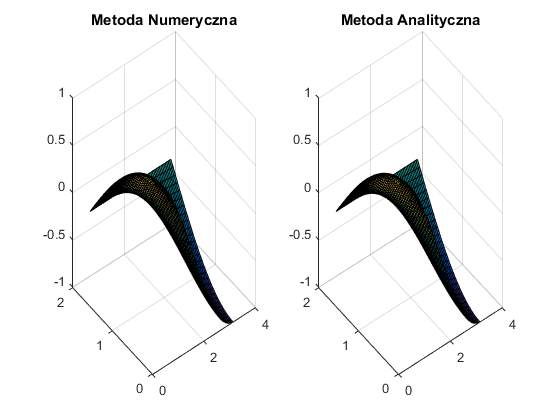
\includegraphics[width=0.8\textwidth]{Lab6/charts/jacobi/zad2/55.png}
	\end{center}
\end{figure}

Liczba wykonanych iteracji $ = 1058 $

Czas wykonywania algorytmu $ = 0.753 s$


\subsection{Metoda Gaussa - Seidela	}

Jest to dowolona modyfikacja metody Jacobiego, a wprowadzana zmiana niemal dwukrotnie przyspiesza tempo zbieżności.

W metodzie tej wartości przybliżone rozwiązania numerycznego są poprawiane w węzłach siatki zgodnie z ustalonym przez cały proces iteraycjny porządkiem.

Dowolne pierwsze przybliżenie (poprawione):

$$u_{i,j}^{(n+1)} = \frac{1}{4}(u_{i+1,j}^{(n)} + u_{i-1,j}^{(n+1)} + u_{i,j+1}^{(n)} + u_{i,j-1}^{(n+1)}) - \frac{1}{4}h^2f_{i,j}$$

Schemat ten jest pozornie niejawny, ale w rzeczywistości uwzględnia on w kroku $n+1$ poprawkę wcześniej już obliczoną.

\subsection{Algorytm}

a)

//kod gs1

b)

//kod gs2

\subsection{Wykresy}

a)

Dla n = 5:

\begin{figure}[!ht]
	\begin{center}
		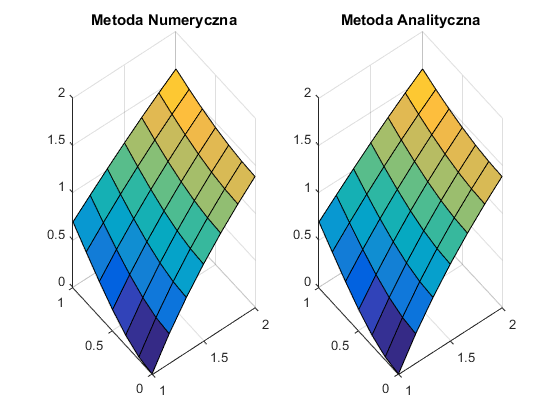
\includegraphics[width=0.8\textwidth]{Lab6/charts/gs/zad1/5.png}
	\end{center}
\end{figure}

Liczba wykonanych iteracji $ = 21 $

Czas wykonywania algorytmu $ = 0.167 s$

Dla n = 15:

\begin{figure}[!ht]
	\begin{center}
		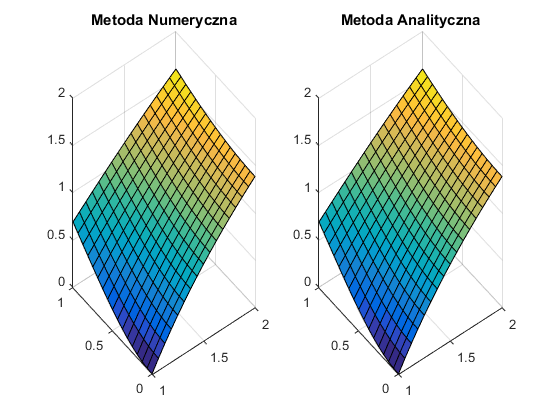
\includegraphics[width=0.8\textwidth]{Lab6/charts/gs/zad1/15.png}
	\end{center}
\end{figure}

Liczba wykonanych iteracji $ = 75 $

Czas wykonywania algorytmu $ = 0.181 s$

Dla n = 30:

\begin{figure}[!ht]
	\begin{center}
		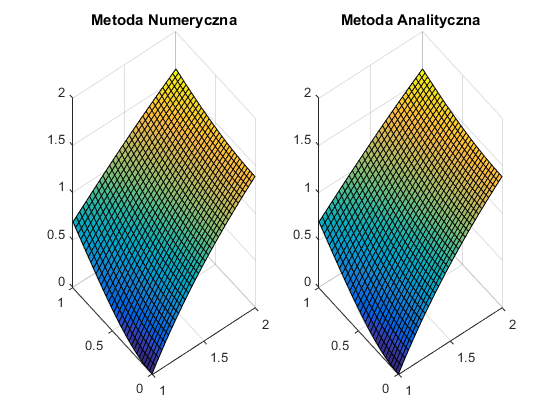
\includegraphics[width=0.8\textwidth]{Lab6/charts/gs/zad1/30.png}
	\end{center}
\end{figure}

Liczba wykonanych iteracji $ = 232 $

Czas wykonywania algorytmu $ = 0.241 s$

Dla n = 50:

\begin{figure}[!ht]
	\begin{center}
		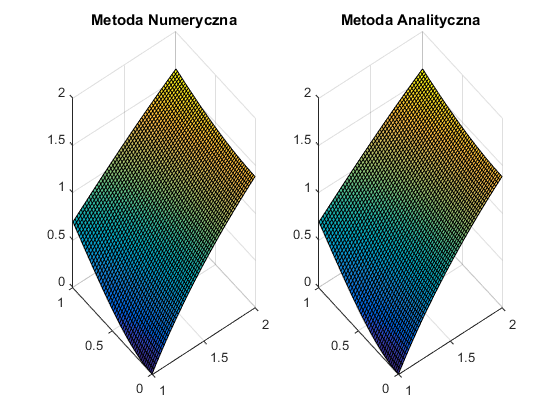
\includegraphics[width=0.8\textwidth]{Lab6/charts/gs/zad1/50.png}
	\end{center}
\end{figure}

Liczba wykonanych iteracji $ = 485 $

Czas wykonywania algorytmu $ = 0.548 s$

b)

Dla n = 5:

\begin{figure}[!ht]
	\begin{center}
		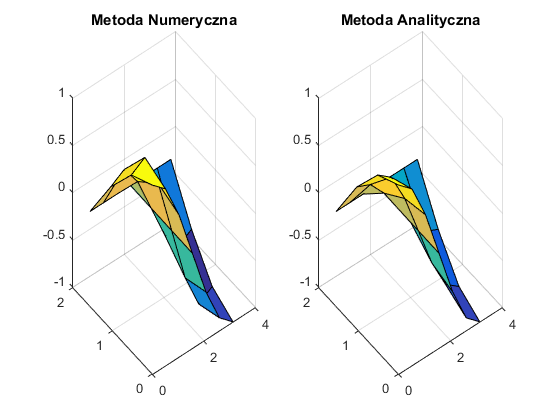
\includegraphics[width=0.8\textwidth]{Lab6/charts/gs/zad2/5.png}
	\end{center}
\end{figure}

Liczba wykonanych iteracji $ = 14 $

Czas wykonywania algorytmu $ = 0.177 s$

Dla n = 15:

\begin{figure}[!ht]
	\begin{center}
		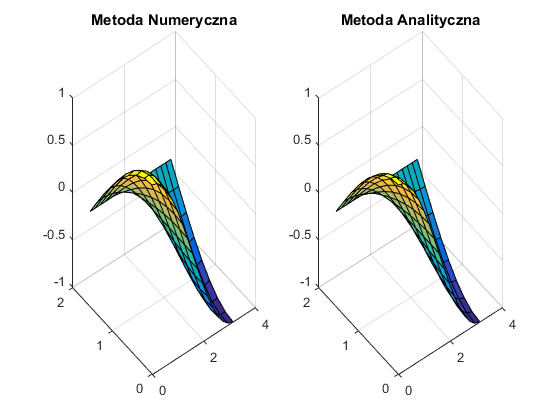
\includegraphics[width=0.8\textwidth]{Lab6/charts/gs/zad2/15.png}
	\end{center}
\end{figure}

Liczba wykonanych iteracji $ = 78 $

Czas wykonywania algorytmu $ = 0.175 s$

Dla n = 35:

\begin{figure}[!ht]
	\begin{center}
		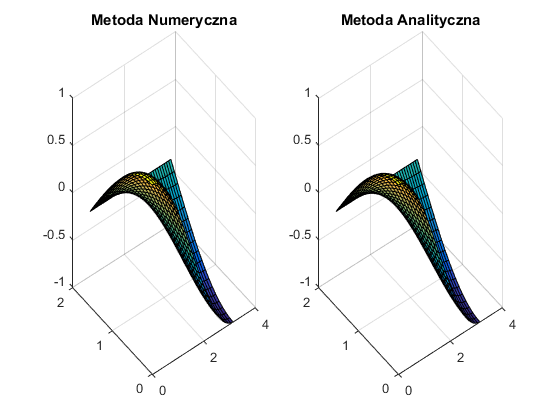
\includegraphics[width=0.8\textwidth]{Lab6/charts/gs/zad2/35.png}
	\end{center}
\end{figure}

Liczba wykonanych iteracji $ = 304 $

Czas wykonywania algorytmu $ = 0.242 s$

Dla n = 55:

\begin{figure}[!ht]
	\begin{center}
		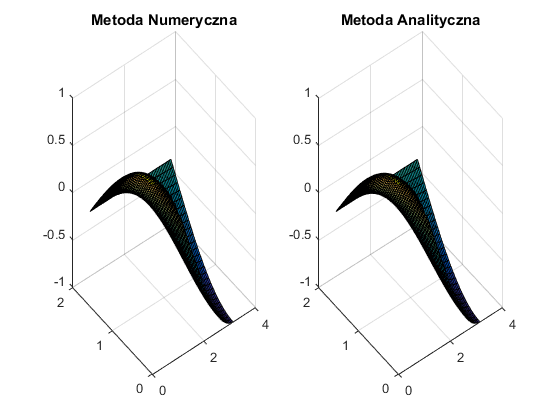
\includegraphics[width=0.8\textwidth]{Lab6/charts/gs/zad2/55.png}
	\end{center}
\end{figure}

Liczba wykonanych iteracji $ = 621 $

Czas wykonywania algorytmu $ = 0.511 s$

\subsection{Metoda nadrelaksacji Younge'a}

Rozważmy modyfikację metody Gaussa $-$ Seidela.

$$u_{i,j}^{(n+1)} = \frac{1}{4}\omega(u_{i+1,j}^{(n)} + u_{i-1,j}^{(n+1)} + u_{i,j+1}^{(n)} + u_{i,j-1}^{(n+1)}) + (1-\omega)u^n_{i,j} - \frac{1}{4}h^2f_{i,j}$$

, gdzie $\omega \hspace{0.1cm} -$ parametr relaksacji

Zauważmy, gdy $\omega = 1$, otrzymujemy metodę Gaussa $-$ Seidela. 

Właściwy wybór parametru relaksacji pozwala na znaczące przyspieszenie zbieżności metody.

Young udowodnił, że wartość optymalna $\omega$ dana jest następującą zależnością:

$$\omega_{opt}=1+\dfrac{\lambda}{(1+\sqrt{1-\lambda})^2}$$

$$\lambda = \dfrac{1}{4}\Big(\cos\Big(\dfrac{\pi}{N}\Big) + \cos\Big(\dfrac{\pi}{M}\Big)\Big)^2$$

, gdzie: M oraz N to liczba elementów, na które podzielono boki

W przypadku innej geometrii niż prostokątna, dla równań Laplace'a i Poissona, $\lambda$ można obliczyć korzystając z tej zależności biorąc wymiar największego prostokąta, który zawiera ten obszar.

Tak wyznaczony parametr relaksacji będzie wyższy niż optymalny, lecz Young udowodnił, że taki nadmiarowy współczynnik, nie zmniejsza znacząco szybkości zbieżności tej metody.

\subsection{Algorytm}

a)

//kod young1

b)

//kod young2

\subsection{Wykresy}

a)

Dla n = 5:

\begin{figure}[!ht]
	\begin{center}
		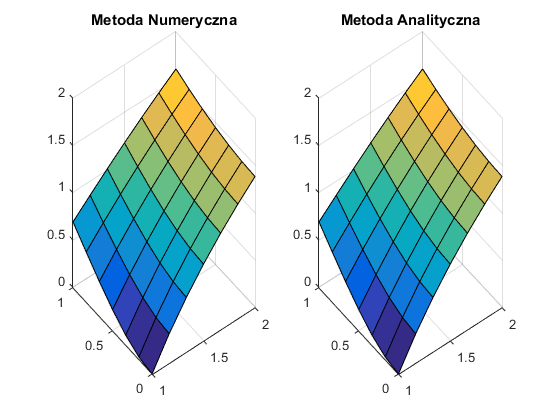
\includegraphics[width=0.8\textwidth]{Lab6/charts/young/zad1/5.png}
	\end{center}
\end{figure}

Liczba wykonanych iteracji $ = 15 $

Czas wykonywania algorytmu $ = 0.183 s$

Dla n = 15:

\begin{figure}[!ht]
	\begin{center}
		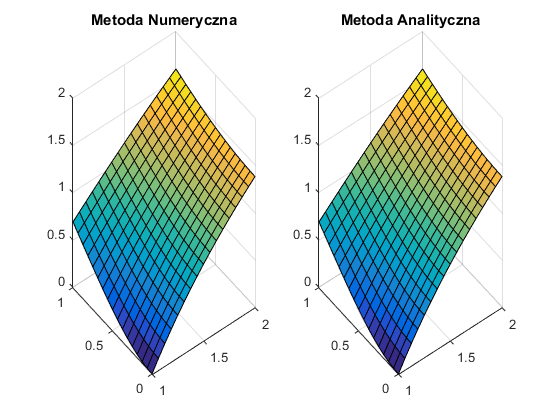
\includegraphics[width=0.8\textwidth]{Lab6/charts/young/zad1/15.png}
	\end{center}
\end{figure}

Liczba wykonanych iteracji $ = 33 $

Czas wykonywania algorytmu $ = 0.181 s$

Dla n = 30:

\begin{figure}[!ht]
	\begin{center}
		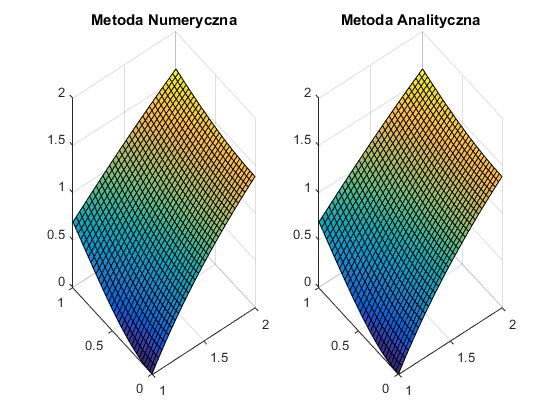
\includegraphics[width=0.8\textwidth]{Lab6/charts/young/zad1/30.png}
	\end{center}
\end{figure}

Liczba wykonanych iteracji $ = 64 $

Czas wykonywania algorytmu $ = 0.197 s$

Dla n = 50:

\begin{figure}[!ht]
	\begin{center}
		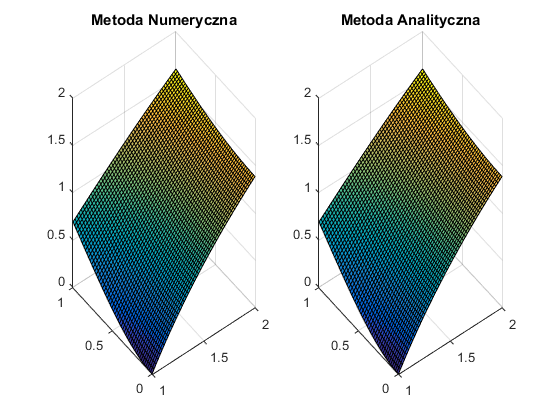
\includegraphics[width=0.8\textwidth]{Lab6/charts/young/zad1/50.png}
	\end{center}
\end{figure}

Liczba wykonanych iteracji $ = 104 $

Czas wykonywania algorytmu $ = 0.269 s$

b)

Dla n = 5:

\begin{figure}[!ht]
	\begin{center}
		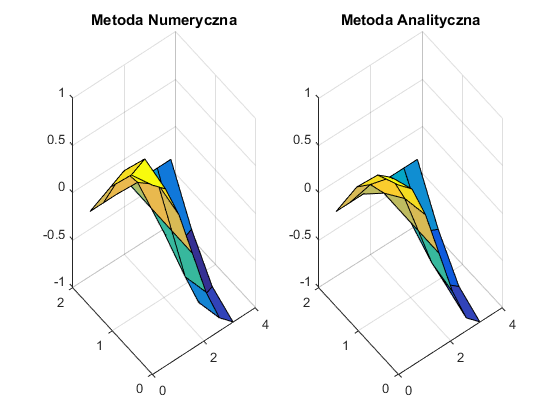
\includegraphics[width=0.8\textwidth]{Lab6/charts/young/zad2/5.png}
	\end{center}
\end{figure}

Liczba wykonanych iteracji $ = 13 $

Czas wykonywania algorytmu $ = 0.176 s$

Dla n = 15:

\begin{figure}[!ht]
	\begin{center}
		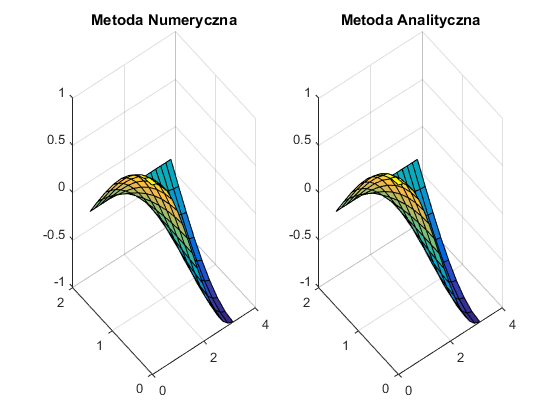
\includegraphics[width=0.8\textwidth]{Lab6/charts/young/zad2/15.png}
	\end{center}
\end{figure}

Liczba wykonanych iteracji $ = 28 $

Czas wykonywania algorytmu $ = 0.180 s$

Dla n = 35:

\begin{figure}[!ht]
	\begin{center}
		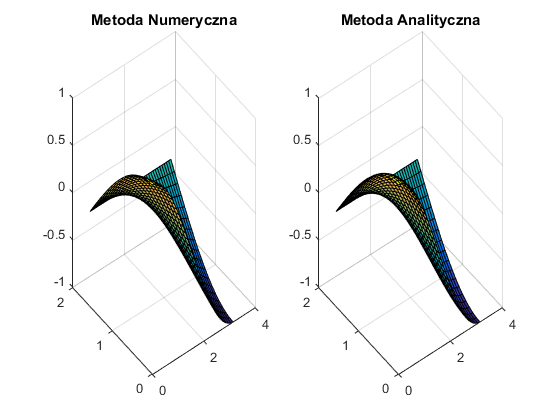
\includegraphics[width=0.8\textwidth]{Lab6/charts/young/zad2/35.png}
	\end{center}
\end{figure}

Liczba wykonanych iteracji $ = 54 $

Czas wykonywania algorytmu $ = 0.192 s$

Dla n = 55:

\begin{figure}[!ht]
	\begin{center}
		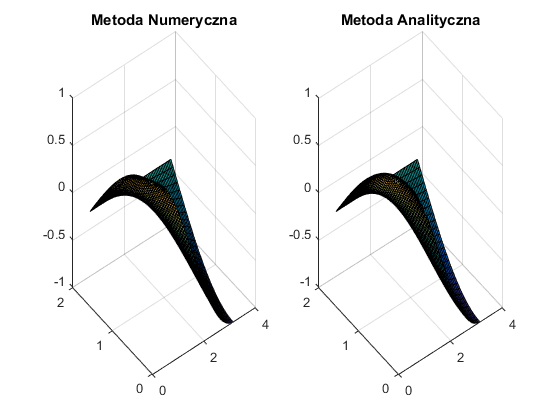
\includegraphics[width=0.8\textwidth]{Lab6/charts/young/zad2/55.png}
	\end{center}
\end{figure}

Liczba wykonanych iteracji $ = 84 $

Czas wykonywania algorytmu $ = 0.227 s$

\begin{figure}[!ht]
	\begin{center}
		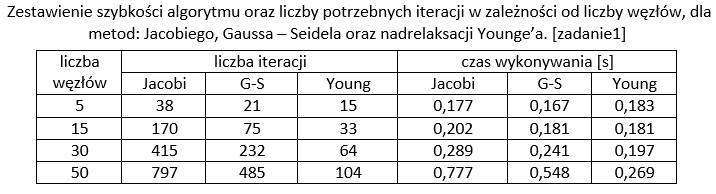
\includegraphics[width=1\textwidth]{Lab6/charts/zestawienie_zad1.png}
	\end{center}
\end{figure}

\begin{figure}[!ht]
	\begin{center}
		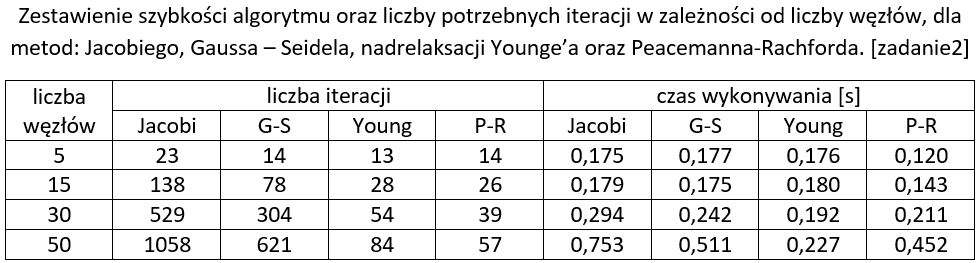
\includegraphics[width=1\textwidth]{Lab6/charts/zestawienie_zad2.png}
	\end{center}
\end{figure}